\subsection{与复极化几何量子化的比较}\label{branecp}

现在考虑 $Y$ 有全纯极化 $\varPi$ 并在 $M$ 上诱导复结构 $\J$ 时 $M$ 的膜量子化。如第 \ref{scbq} 节所述，全纯极化成对出现 $\varPi,\varPi'$，在 $M$ 上诱导相反的复结构 $\J,-\J$。二者不能同时为 Kähler，故我们简要讨论复极化不必为 Kähler 时的几何量子化。

若 $M$ 有预量子线丛 $\frL$ 及由复结构 $\J$ 定义的极化，则几何量子化一般把此数据对应于上同调 $H^r_\J(M,K_M^{1/2}\otimes\frL)$，$0\le r\le n=\dim_\C M$。记号 $H^r_\J$ 指复结构 $\J$ 下的层上同调（必要时把 $K_M$ 写作 $K_{M,\J}$）。复极化一般由整数 $r_0$ 刻画，它定义为 $M$ 上任一点 $m$ 的切空间中辛形式 $\omega$ 为负的复方向数。（此数对 $M$ 中任一点相同，因 $\omega$ 处处非退化。）极化为 Kähler 当且仅当 $r_0=0$。这是最重要、研究最多的情形。Kähler 极化时，若充分接近经典极限（即辛形式 $\omega$ 的周期充分大），则上同调 $H^r_\J(M,K_M^{1/2}\otimes\frL)$ 对 $r>0$ 消失。此时几何量子化的配方归结为：量子态的 Hilbert 空间为
\be\label{defq} \H_\gq=H^0_\J(M,K_M^{1/2}\otimes\frL),\ee
带自然的 Hermite 内积
\be\label{mellow}\la\chi,\psi\ra=\int_M\d\mu\,\bar\chi\psi,\ee
其中 $\mu$ 是 $M$ 上的辛测度。复极化非 Kähler 时，须考虑 $r\ne0$ 的 $H^r_\J(M,K_M^{1/2}\otimes\frL)$。只要把 $H^r_\J(M,K_M^{1/2}\otimes\frL)$ 解释为 $M$ 上取值于 $K_M^{1/2}\otimes\frL$ 的 $\ltwo$ 调和 $(0,r)$-形式空间，Hilbert 空间结构 (\ref{mellow}) 的定义对任意 $r$ 都有意义。只要恰有一个 $r$ 使 $H^r_\J(M,K_M^{1/2}\otimes\frL)$ 非零，此空间就是量子 Hilbert 空间的合理候选，几何量子化也就给出 $M$ 量子化的合理答案。若充分接近经典极限，可望相关的 $\ltwo$ 上同调只在一个 $r$ 值非零，即 $r=r_0$。若上同调在多于一个 $r$ 值非零，则用复极化 $\J$ 的几何量子化是否真给出合理答案就值得怀疑了。

特殊情形是 $\J$ 定义 Kähler 极化，而我们要用复结构 $-\J$ 量子化 $M$。对 $-\J$，$\omega$ 负定，故 $r_0=n=\dim_\C M$。Hodge 理论把 $H^n_{-\J}(M,K_{M,-\J}^{1/2}\otimes\frL)$ 等同于 $H^0_\J(M,K_{M,\J}^{1/2}\otimes\frL)$，故用复结构 $-\J$ 的几何量子化等价于用复结构 $\J$ 的几何量子化。更一般地，对任意 $r$，Hodge 理论给出同构 $H^r_\J(M,K_{M,\J}^{1/2}\otimes\frL)\cong H^{n-r}_{-\J}(M,K_{M,-\J}^{1/2}\otimes\frL)$，故基于 $-\J$ 的几何量子化总等价于基于 $\J$ 的几何量子化。

本节目标是在某些假设下比较膜量子化与几何量子化。在一定条件下，我们将证明（不论 $r_0$ 取何值）几何量子化所考虑的上同调群承载可观测量代数 $\A=\Hom(\B_\cc,\B_\cc)$ 的作用，而该代数在膜量子化中作用。我们还将更直接地证明：Kähler 极化情形下，$\H=\Hom(\B,\B_\cc)$ 与 $\H_\gq$ 作为向量空间有自然等同。此等同\emph{不}保证延拓为 Hilbert 空间结构之间的等价。当存在适当的反线性对称时，膜量子化给出 $\H$ 上 Hilbert 空间结构的定义，但没有明显理由认为该结构等价于 (\ref{mellow}) 那样的初等公式。第 \ref{flatg} 节将考虑的例子提示，事情并不那么简单。

为执行此计划，假定 $Y$ 配有全纯极化 $\varPi$ 与投影 $\pi:Y\to W$。更具体地，假定 $Y$ 是按第 \ref{shifted} 节从全纯线丛 $\L\to W$（或更一般地，线丛复幂的形式张量积\footnote{此处及下文令 $\hbar=1$。}$\L=\otimes_{s=1}^k\L_s^{\lambda_s}$）构造的扭余切丛。

先考虑 $M$ 紧的情形。此时 $\pi(M)$ 必为整个 $W$（若是 $W$ 的真开子集则不紧）。故 $M$ 是 $\pi:Y\to W$ 的非全纯截面，这保证限制到 $M$ 上时 $\pi$ 是 $M$ 与 $W$ 之间的同构。由于 $\pi$ 的纤维可缩，这表明 $Y$ 可缩到 $M$ 上。为定义支撑在 $M$ 上的拉格朗日膜 $\B$，首先 $M$ 应为拉格朗日的，即 $\Im\Omega$ 限制到 $M$ 为零。由于 $Y$ 可缩到 $M$，这表明上同调类 $[\Im\Omega]$ 为零。还需预量子线丛 $\frL\to M$，曲率为 $\Re\Omega$。这要求 $c_1(\frL)=[\Re\Omega]/2\pi$。合并两式，需要对实际线丛 $\frL$ 有 $[\Omega]/2\pi=c_1(\frL)$。回看式 (\ref{jnko}) 可知，这些条件可满足当且仅当 $\L$ 作为实际线丛存在；此时应取 $\frL=\L$。更确切地说，$\L$ 只在可张量平坦线丛的意义下定义；定义 $\frL$ 时须作具体选择。

$W_0=\pi(M)$ 也可能是 $W$ 的真开子集。此时条件较宽松：只要求限制到 $\pi^{-1}(W_0)$ 时 $[\Im\Omega]$ 为零，且 $\L$ 作为实际线丛存在。

可用第 \ref{example} 节的例子说明两种情形的差别。先考虑 $x^2+y^2+z^2=j^2$ 定义的复流形 $Y$，复辛形式 $\Omega=\d x\d y/z$。设 $j^2>0$，用同一方程 $x^2+y^2+z^2=j^2$ 且 $x,y,z$ 为实定义 $M$。如第 \ref{scbq} 节所示，$\pi:M\to W$ 是从 $M\cong S^2$ 到 $W\cong\bCP^1$ 的同构。故 $Y$ 可缩到 $M$。简单计算给出
\be\label{shortc} \int_M\Omega=4\pi j. \ee
故存在线丛 $\L\to W\cong\bCP^1$ 使 $c_1(\L)=[\Omega]/2\pi$ 的条件是 $j\in\frac12\Z$。此时线丛 $\L$ 存在，且 $\L=\O(2j)$。取 $\frL=\L$ 作 $M$ 的预量子线丛；定义支撑在 $M$ 上的膜 $\B$，其 $\CP$ 丛为 $\frL^{-1}$。

把此与表面相似的例子比较：由 $x^2-y^2-z^2=j^2$ 定义的复流形 $Y'$，仍取 $\Omega=\d x\d y/z$、$j^2>0$。用同一方程 $x^2-y^2-z^2=j^2$ 且 $x,y,z$ 为实定义 $M$，并加条件 $x>0$。与前一情形的差别是 $M$ 可缩；如第 \ref{scbq} 节所解释，$\pi:M\to W$ 把 $M$ 等同于 $W\cong\bCP^1$ 中的开上半平面（或上半球面）。故 $\L$ 限制到 $M$ 上作为线丛存在的条件平凡，对任意实 $j$ 都可取 $\L=\O(2j)$。预量子线丛于是也是 $\frL=\O(2j)$。作为 $\bCP^1$ 上的线丛这不合理，但在 $M$ 上合理。

检验这类例子中膜量子化与几何量子化预言相同物理态空间（但未必相同 Hilbert 空间结构）的一个办法如下。自然作用在 $\H=\Hom(\B,\B_\cc)$ 上的代数是 $\A=\Hom(\B_\cc,\B_\cc)$。沿 $W$ 层化后，可把它看作代数层而非单个代数。第 \ref{shifted} 节已证明 $\A$ 是作用在 $K_M^{1/2}\otimes\frL$ 上的全纯微分算符层（当然在复结构 $\J$ 下）。显然此代数作用在 $K_M^{1/2}\otimes\frL$ 的全纯截面上；同样显然的是，由于全纯微分算符与 $\bar\partial$ 算符交换，同一代数作用在取值于 $K_M^{1/2}\otimes\frL$ 的所有 $\bar\partial$ 上同调群上。于是几何量子化定义的物理态空间确实承载膜量子化中预期的可观测量代数作用。

对涉及 $Y$ 或 $Y'$ 的简单例子，可把这些陈述完全显式化。$Y$ 情形下，可观测量代数由式 (\ref{throps}) 的三个算符 $t_+,t_-,t_3$ 生成。对 $j\in\frac12\Z$，物理 Hilbert 空间 $\H=H^0(\bCP^1,\O(2j-1))$ 的维数为 $2j$；这 $2j$ 个态构成 $\SU(2)$ 的自旋 $j-\frac12$ 不可约表示。在式 (\ref{throps}) 的表示中，态是 $q$ 的次数 $\le 2j-1$ 的多项式；$t_+,t_-,t_3$ 作为熟悉的 $\mathfrak{su}(2)$ 生成元作用在这些态上。（例如 $t_3$ 的本征值为 $j-\frac12,j-\frac32,\cdots,-j+\frac12$。）显然，这一切只因为 $2j$ 是整数才有意义。$Y'$ 情形类似，但此时 $t_+,t_-,t_3$ 生成 $\PSL(2,\R)$（或其覆盖群，取决于 $j$）的酉表示而非 $\SU(2)$ 的，作用在 $M\cong\mathcal H$ 上 $\O(2j-1)$ 的全纯截面上。

若 $\J$ 是 Kähler 极化，可更直接地论证 $\H_\gq$ 与 $\H=\Hom(\B,\B_\cc)$ 相同。仿照第 \ref{ccb} 节的构造。令 $w$ 为 $M$ 中点，$F$ 为含 $w$ 的 $\varPi$ 纤维。如常定义支撑在 $F$ 上、$\CP$ 丛平凡的膜 $\F$，并通过复合 $\Hom(\B_\cc,\F)$ 与 $\Hom(\F,\B)$ 中的适当元素，得到 $\H'=\Hom(\B_\cc,\B)$ 中的元素。如前，$\Hom(\B_\cc,\F)\cong H^0(F,K_F^{1/2})$。选取参数化 $w$ 附近 $M$ 与 $F$ 的局部坐标 $\vec q$ 与 $\vec p$，使 $\Omega=\sum_i\d p_i\d q^i$，则可取 $H^0(F,K_F^{1/2})$ 中在 $w$ 处限制为 $\alpha=(\d\vec p)^{1/2}$ 的元素。由于 $\F$ 与 $\B$ 交于唯一点 $w$，$\Hom(\F,\B)$ 是一维的，是 $\frL^{-1}|_w$ 的拷贝，即 $\B$ 的 $\CP$ 丛在 $w$ 处的纤维。故对任意 $\beta\in\frL^{-1}|_w$，有 $\Hom(\F,\B)$ 中的元素。复合 $\Hom(\B_\cc,\F)$ 与 $\Hom(\F,\B)$ 的这些元素，得 $\psi'(w;\alpha,\beta)\in\H'=\Hom(\B_\cc,\B)$。$\psi'$ 全纯依赖于 $w$；这将在第 \ref{flatcon} 节解释。如第 \ref{ccb} 节，若 $\Psi$ 是 $\H$ 中任一元，可定义 $A$-模型双线性配对 $f(w;\alpha,\beta)=(\psi'(w;\alpha,\beta),\Psi)$。再乘以 $\sqrt{\d\vec q}\,\beta^{-1}$ 以抵消对 $\alpha,\beta$ 选择的依赖。故定义
\be\label{zofo}\h\Psi=\sqrt{\d\vec q}\,\beta^{-1}f(w;\alpha,\beta). \ee
由于因子 $\sqrt{\d\vec q}$ 与 $\beta^{-1}$，$\h\Psi$ 取值于 $K_M^{1/2}\otimes\frL$ 在 $w$ 处的纤维。此外 $\h\Psi$ 全纯依赖于 $w$，因为 $\psi'(w;\alpha,\beta)$ 全纯依赖于 $w$。简言之，此构造定义从膜量子化的物理态空间 $\H$ 到几何量子化中对应物 $\H_\gq$ 的映射。我们预期此映射恰在 $\varPi$ 诱导的 $M$ 的复极化为 Kähler 时非零，且此时为同构。

膜量子化给出定义 $\H$ 的 Hermite 结构的配方，但很难把此配方化为显式公式。一般配方已在第 \ref{hermitian} 节解释。为在当前背景下使其稍显式，可如下进行。首先，在 $\H$ 或其对偶空间 $\H'$ 上定义 Hermite 结构等价，且后者更方便。我们将定义 $\psi'(w;\alpha,\beta)$ 与用另一组选择 $\t w,\t\alpha,\t\beta$ 定义的类似态 $\psi'(\t w;\t\alpha,\t\beta)\in\H'$ 的内积。一般配方说，Hermite 内积由 $A$-模型双线性配对对其中一个态作用反线性算符 $\Theta_\tau$ 得到：$\la\psi'(w;\alpha,\beta),\psi'(\t w;\t\alpha,\t\beta)\ra=(\Theta_\tau\psi'(w;\alpha,\beta),\psi'(\t w;\t\alpha,\t\beta))$。反线性映射 $\Theta_\tau$ 把全纯极化 $\varPi$ 与其共轭 $\varPi'$ 交换。特别地，$\Theta_\tau$ 把 $\F$ 映到支撑在含 $w$ 的 $\varPi'$ 纤维 $F'$ 上的膜 $\F'$。$\Theta_\tau$ 同样把复合得到 $\psi'(w;\alpha,\beta)$ 的 $\Hom(\B_\cc,\F)$ 与 $\Hom(\F,\B)$ 中元素，映到 $\Hom(\B,\F')$ 与 $\Hom(\F',\B_\cc)$ 中元素，其复合为 $\Theta_\tau\psi'(w;\alpha,\beta)\in\H=\Hom(\B,\B_\cc)$。此态与 $\psi'(w;\alpha,\beta)$ 的 $A$-模型配对，如前例，可由矩形上的路径积分表示：$\psi'(\t w;\t\alpha,\t\beta)$ 在顶部，$\Theta_\tau\psi'(w;\alpha,\beta)$ 在底部（图 \ref{newrectangle}）。遗憾的是，矩形上的路径积分难以计算。它约化为三角形乘积之和（图 \ref{newrectangle}(b)），但即使这样，也很可能得不到一般公式。

\begin{figure}[htbp]
 \centering
 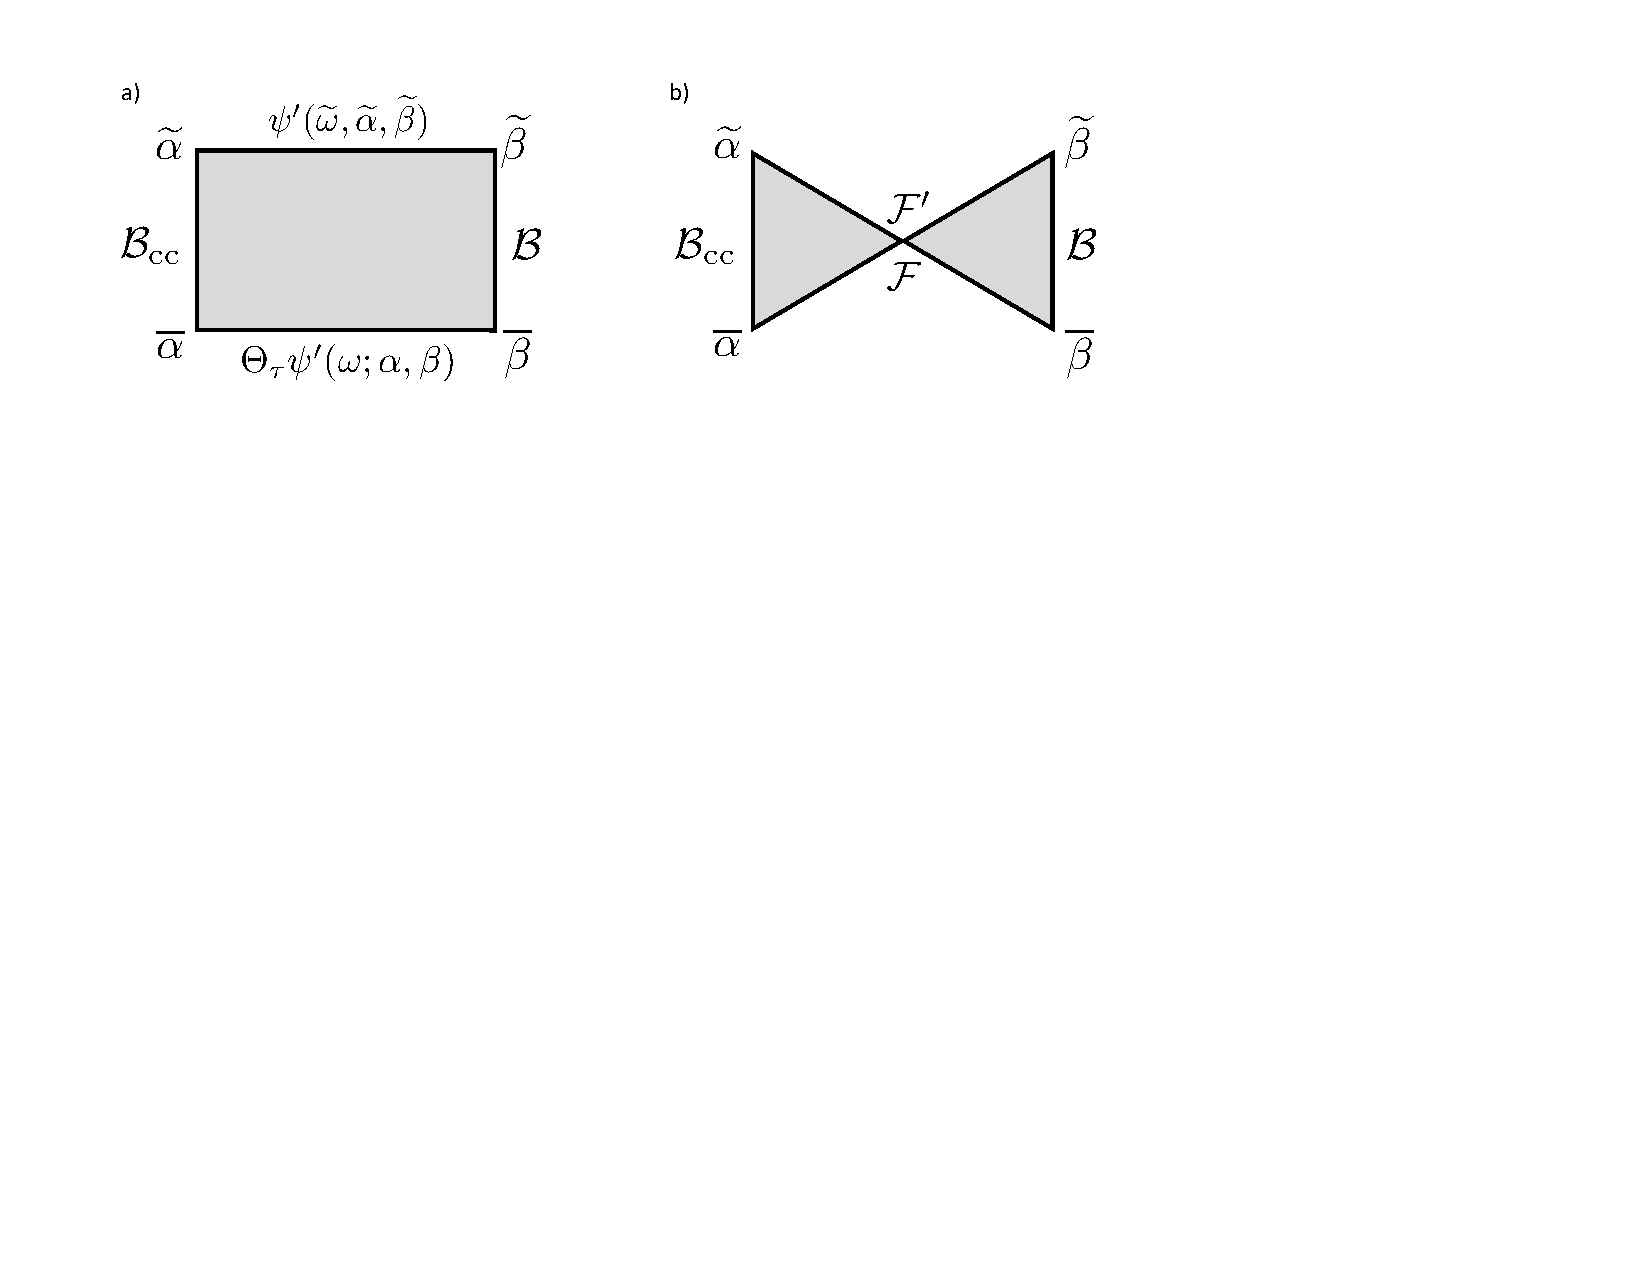
\includegraphics[width=0.86\textwidth]{figures/5.pdf}
 \caption{\small (a) 带所示边界条件的矩形上的路径积分可用于计算内积。(b) 矩形可约化为在顶点粘合的三角形之并。计算相应路径积分时，须对穿过该顶点传播的态求和。}
 \label{newrectangle}
\end{figure}

值得注意的一点是：与余切丛的讨论不同，态 $\psi'(w;\alpha,\beta)$ 可归一化。令 $w=\t w$ 时图 \ref{newrectangle} 不出现奇点。在当前背景下不应期待遇到 delta 函数态，因为例如 $M$ 紧时物理态空间有限维，不会有 delta 函数态这种东西。
